\documentclass[5pt, compress]{beamer}

\usepackage[T1]{fontenc} % Use 8-bit encoding that has 256 glyphs
\usepackage{fourier} % Use the Adobe Utopia font for the document - comment this line to return to the LaTeX default
\usepackage[frenchb]{babel} % English language/hyphenation
\usepackage[none]{hyphenat}
%\usepackage[utf8x]{inputenc}
\usepackage{booktabs}
\usepackage[scale=2]{ccicons}
\usepackage{scrextend}
\changefontsizes{10pt}

\usetheme[usetitleprogressbar, nooffset]{m}

\usepackage{minted}
\usepackage{tcolorbox}
\usepackage{listings}
\usepackage{nameref}
\usepackage{amsmath,amsfonts,amsthm} % Math packages
\usepackage{arydshln}

\makeatletter
\newcommand*{\currentname}{\@currentlabelname}
\makeatother

\usepgfplotslibrary{dateplot}

\usemintedstyle{trac}
\setbeamertemplate{itemize item}[square]
%\setbeamertemplate{itemize subitem}[square]

\title{\huge Soutenance de mémoire}
\subtitle{\normalsize Maitre de stage: Cédric Bastoul\\Lieu: Équipe ICPS, ICube}
\date{Lundi 22 juin 2015}
\author{\huge Thomas Kuntz}
\institute{\normalsize Master RISE, Unistra, Strasbourg, France}


%20min → 20 slide contenus + 5 slide titre/contenu
\begin{document}
%Code pour example polyédral
\defverbatim[colored]\codeExample{
\tiny\tt
\vspace{-0.3cm}
\begin{lstlisting}
for (i = 0; i < 3; i++)
  for (j = 0; j < 3; j++)
    z[i+j] += x[i] * y[j];
\end{lstlisting}
\vspace{-0.3cm}
}
\defverbatim[colored]\codeExampleParallel{
\tiny\tt
\vspace{-0.3cm}
\lstset{emph={parallel},emphstyle=\bf\color{red}}
\begin{lstlisting}
#pragma omp parallel for private(p, i)
for (p = 0; p < 5; p++) {
  for (i = max(0,p-2); i <= min(2,p); i++) {
    z[p] += x[i] * y[p-i];
\end{lstlisting}
\vspace{-0.3cm}
}

    \maketitle    

%\begin{alertblock}{Un bloc très alerte}
%\begin{exampleblock}{Un bloc exemplaire}

\section{Présentation du laboratoire}
    \begin{frame}{\currentname}
        \begin{block}{ICube}
            \begin{itemize}
                \item Laboratoire créé en 2013
                \item Fusion de 4 laboratoires (LSIIT, InESS, IMFS, IPB-LINC)
                \item Co-tutelle de l'Université de Strasbourg, du CNRS, de l'ENGEES
                    et l'INSA de Strasbourg
                %\item Champs d'applications privilégiés: Imagerie, Ingénierie pour la 
                    %santé et l'environnement et le développement durable.
                \item 4 départements : 
                    D-IRTS (Imagerie, Robotique, Télédetection \& Santé),
                    D-ESSP (Électronique du Solide, Systèmes \& Photonique), D-M (Mécanique)
                    \textbf{et D-IR (Informatique Recherche)}.
                %\item Dirigé par M. de Mathelin.
            \end{itemize}
        \end{block}
        \begin{minipage}{0.19\linewidth}
            \center
        
\includegraphics[height=2em]{./images/ICube}
        \end{minipage} \hfill
        \begin{minipage}{0.19\linewidth}
            \center
        
\includegraphics[height=2em]{./images/Unistra}
        \end{minipage} \hfill
        \begin{minipage}{0.19\linewidth}
            \center
        
\includegraphics[height=2em]{./images/CNRS}
        \end{minipage} \hfill
        \begin{minipage}{0.19\linewidth}
            \center
        
\includegraphics[height=2em]{./images/ENGEES}
        \end{minipage} \hfill
        \begin{minipage}{0.19\linewidth}
            \center
        
\includegraphics[height=2em]{./images/INSA}
        \end{minipage}
    \end{frame}
    \begin{frame}{\currentname}
        \begin{block}{ICPS}
            \begin{itemize}
                \item Une des 5 équipes du D-IR
                \item Recherches portées par le calcul scientifique/de haute performance
                \item Emphase sur l'optimisation et parallélisation de programmes
                \item Partenaire du projet CAMUS : 
                    \begin{itemize}
                        \item Techniques de parallélisation et d’optimisation automatiques
                        \item Méthodes de preuves et de certification.
                    \end{itemize}

                %\item Projet Camus (Inria): Axée sur la recherche de techniques de parallélisation
                    %et d’optimisation automatiques,
                    %ainsi que des méthodes de preuves et de certification,
                    %pour l’exploitation efficace des processeurs multi-coeurs existants et à venir.
            \end{itemize}
        \end{block}
    \end{frame}

\section{Présentation du sujet et de la problématique}
    \begin{frame}{\currentname}
        \begin{block}{Problématiques}
            \vspace{-1em}
            \begin{itemize} \itemsep0em
                \item {Compilation polyédrique couteuse pour codes longs/complexes}
                \item {Optimisation non satisfaisante des statements partageant une affinité.}
            \end{itemize}
        \end{block}

        \pause

        \begin{block}{Buts du stage}
            \vspace{-1em}
            \begin{itemize} \itemsep0em
                \item {Profilage des propriétés d'optimisation d'un statement} 
                    \begin{itemize}
                        \item Carte d'identité
                        \item Travaux préliminaires pour un futur optimisateur.
                    \end{itemize}
                \item {Agrégation de statements ayant une certaine affinité}
                    \begin{itemize}
                        \item {Réduire la complexité des techniques polyédriques}
                        \item {Guider les optimisateurs à faire les bons choix.}
                    \end{itemize}
            \end{itemize}
        \end{block}
    \end{frame}

%\section{Motivations}
    %\begin{frame}{\currentname}
        %conventional_beamforming
    %\end{frame}

\section{Méthodologie du stage}
    \begin{frame}{\currentname}
        \begin{itemize}\itemsep1em
            \item \alert<+>{Apprentissage du modèle polyédrique}
            \item \alert<+>{Étudier le moyen de caractériser et modéliser les propriétés d'un statement}
            \item \alert<+>{Étudier le moyen de caractériser et noter l'affinité entre 2 statements}
            \item \alert<+>{Étudier et trouver des stratégies d'agrégation}
            \item \alert<+>{Implémentation, expérimentations et benchmarks.}
        \end{itemize}
    \end{frame}

\section{Présentation du modèle polyédrique}
    \begin{frame}{\currentname}
\vspace{-1.5em}
  \begin{center}
  \begin{tabular}{lc}
  & \hspace{-0.6cm}\begin{minipage}{3.3cm}
  \begin{beamerboxesrounded}[shadow=true]{}
  \codeExample
  \end{beamerboxesrounded}
  \end{minipage} \\

  \begin{minipage}{2cm}
      {\hbox{\textbf{1} Représention sous}\hbox{forme polyédrique}}
  \end{minipage} &  \hspace{-0.7cm}$\Downarrow$ \\ 

  \noalign{\vspace{-.2cm}}
  &
  \begin{minipage}{3cm}
  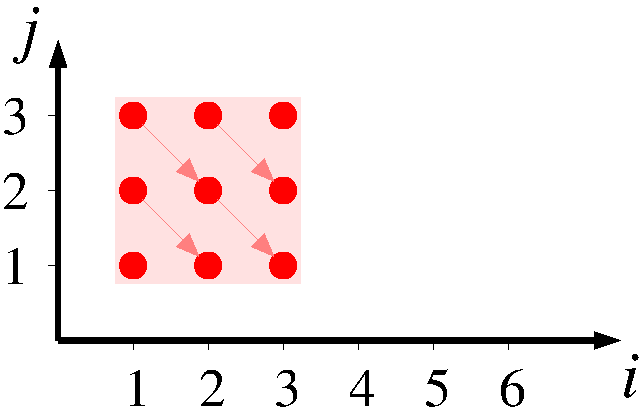
\includegraphics[width=2.2cm]{./images/transfo1reddep.pdf}
  \end{minipage}  \\

  \begin{minipage}{2cm}
      {\hbox{\textbf{2} Transformations de}\hbox{la forme polyédrique}}
  \end{minipage} & \hspace{-0.7cm}$\Downarrow$ \\ 

  \noalign{\vspace{-.2cm}}
  &
  \begin{minipage}{3cm}
  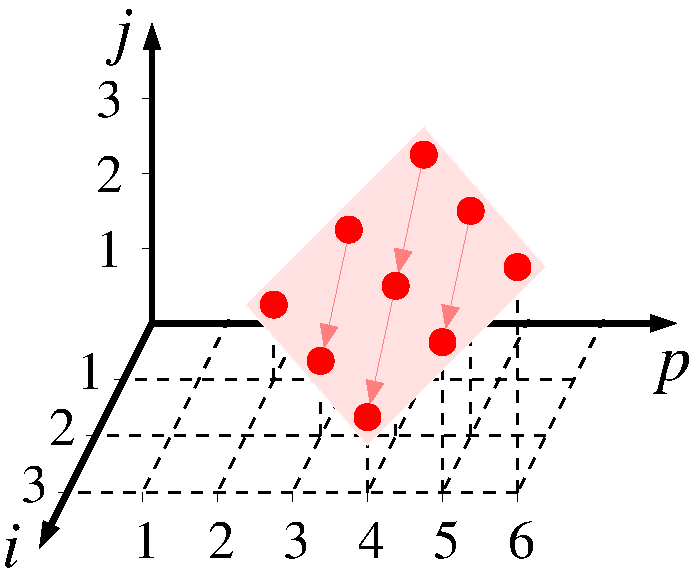
\includegraphics[width=2.4cm]{./images/transfo2reddep.pdf}
  \end{minipage}\\

  \begin{minipage}{2cm}
  {\hbox{\textbf{3} Génération du code}}
  \end{minipage} & \hspace{-0.7cm}$\Downarrow$ \\

  & \hspace{-0.7cm}\begin{minipage}{5.6cm}
  \begin{beamerboxesrounded}[shadow=true]{}
  \codeExampleParallel
  \end{beamerboxesrounded}
  \end{minipage}
  \end{tabular}
  \end{center}
    
    \end{frame}
    \begin{frame}{Relations polyédriques}
        Modèle de relation polyédrique :
        \begin{center}
            $ \mathcal{R} = \bigcup\limits_i \mathcal{R}_i(\vec{p})= \left\{
                \vec{x}_{in} \rightarrow \vec{x}_{out}
                \ \middle| \ 
                R_i \times \left(\begin{array}{c}
                    \vec{x}_{in} \\
                    \vec{x}_{out} \\
                    \vec{p} \\
                    1
            \end{array} \right) \geq \vec{0}
            \right\}$
        \end{center}

        \pause
        \vspace{2em}

        Une représentation polyédrique d'un \textit{statement} comprend ses :
        \begin{itemize}\itemsep0em
            \vspace{-1em}
            \item \textit{Domain Relations} : définit l'ensemble des itérations
            \item \textit{Scattering Relations} : ordonnance les \textit{statements}
            \item \textit{Access Relations} : définit les accès mémoires
            \end{itemize}

            OpenScop : format de fichier/bibliothèque de manipulation polyédrique → pont.\\
            Periscop : suite logiciel d'outils polyédriques basés sur OpenScop.
    \end{frame}
    %\begin{frame}{OpenScop et Periscop}
        %OpenScop est un framework fournissant :
        %\begin{itemize}\itemsep0em
            %\vspace{-1em}
            %\item Un format de fichier pour la représentation polyédrique de code.
            %\item Une bibliothèque implémentant/manipulant le format.
        %\end{itemize}
        %Pont entre les différents programmes polyédriques.

        %\bigskip
        %\pause

        %Periscop est une suite logiciel d'outils polyédriques basés sur OpenScop :
        %\begin{itemize}\itemsep0em
            %\vspace{-1em}
            %\item Bibliothèque OpenScop.
            %\item Clan.
            %\item Candl.
            %\item CLoog.
            %\item Et d'autres encore...
        %\end{itemize}
    %\end{frame}

    \section{Profilage et affinité des statements}
    \begin{frame}[fragile]
    \small
        \frametitle{Réutilisation de données}
\vspace{-0.2em}
        Réutilisation de données : propriété "textuelle".\\
        Localité de données : réutilisation + bon ordonnancement.
\pause
\vspace{-0.2em}
\begin{tcolorbox}
\begin{minted}[fontsize=\footnotesize]{C}
for(i=0; i<N ; i++)
  for(j=0; j<N ; j++)
    A[i][j] = (A[i][j-1] + A[i][j+1] + A[i-1][j] +
      A[i+1][j] + A[2*i][j] + B[i][j]) / 6.0;
\end{minted}
\end{tcolorbox}
\pause
\vspace{-0.3em}
\begin{minipage}{0.38\linewidth}
    Critères :
    \begin{itemize}\itemsep0.1em
        \item Référence (nom)
        \item Ensemble Uniformément Généré (coef. indices).
        \item Direction de réutilisation (partie constante).
    \end{itemize}
\end{minipage} \hfill
\begin{minipage}{0.59\linewidth}
\center
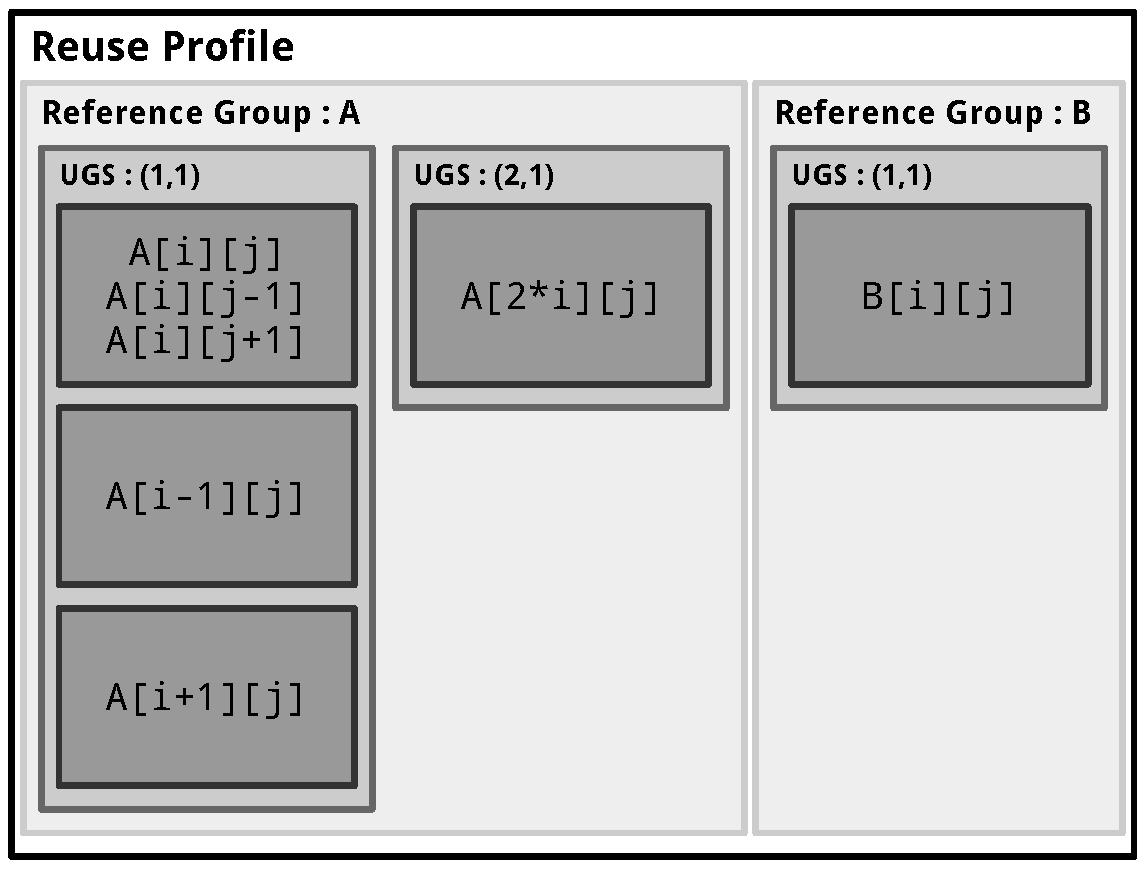
\includegraphics[width=\linewidth]{./images/Reuse_Profile_example1}
\end{minipage}
\end{frame}

\begin{frame}[fragile]
    \frametitle{Réutilisation de données : noter l'affinité de 2 statements}
\only<1>
{
\vspace{-4.7em}
}
\begin{tcolorbox}
\begin{minted}[fontsize=\footnotesize]{C}
for(i=0 ; i<N ; i++)
  for(j=0 ; j<N ; j++) {
    A[i][j] = A[i][j+1] + A[i+1][j] + B[i] + B[2*i]; //S1
    C[i][j] = A[i][j+2];                             //S2
  } 
\end{minted}
\end{tcolorbox}
\pause
\vspace{-0.2em}
\begin{minipage}{0.48\linewidth}
\begin{figure}
    \includegraphics<2>[width=\columnwidth]{images/Reuse_Profile_example2.pdf}
    \includegraphics<3>[width=\columnwidth]{images/Reuse_Profile_example2_bis.pdf}
\end{figure}
\end{minipage}\hfill
\begin{minipage}{0.48\linewidth}
\begin{figure}
    \includegraphics<2>[width=0.7\columnwidth]{images/Reuse_Profile_example3.pdf}
    \includegraphics<3>[width=0.7\columnwidth]{images/Reuse_Profile_example3_bis.pdf}
\end{figure}
\end{minipage}
\pause
\begin{center}
    \small
    Affinité de réutilisation $= \dfrac{\text{Nb accès avec critères égaux}}{\text{Nb total d'accès}}$,\ \ \
    ici $\dfrac{3}{7} \approx 0.43$
\end{center}
\end{frame}
    \begin{frame}{Parallélisme}
        Principe : exécuter plusieurs instances d'un statement en même temps.
        \pause
        \begin{itemize}
            \item \alert<+>{Profilage du statement \textbf{seul}}
            \item \alert<+>{Trouver les boucles parallélisables avec les \textit{Dependence Relations}}
            \begin{minipage}{0.36\linewidth}
            \vspace{0.7em}
                \begin{itemize}
                    \item Conditions d'existence
                    \item Conditions de conflit
                    \item Conditions de causalité.
                \end{itemize}
            \end{minipage} \hfill
            \begin{minipage}{0.63\linewidth}
            \vspace{0.7em}
                \center
            \scalebox{0.45}{
            ${
            \delta_{S,r_S \xrightarrow{d} T,r_T}(\vec{p}) =
                \left\{
                \begin{pmatrix}\vec{\imath}_S \\ \vec{a}_{S,r_S} \end{pmatrix}
                \to
                \begin{pmatrix}\vec{\imath}_T \\ \vec{a}_{T,r_T} \end{pmatrix}
            \middle|
                \left[\begin{array}{c:c|c:c|c:c}
                    D^{\vec{\imath}_S}_{S} & 0 & 0 & 0 & D^{\vec{p}_S}_{S} & D^{c}_{S} \\ \hdashline
                    0 & 0 & D^{\vec{\imath}_T}_{T} & 0 & D^{\vec{p}_T}_{T} & D^{c}_{T} \\ \hline
                    A^{\vec{\imath}_S}_{S,r_S} & A^{\vec{a}_{S,r_S}}_{S,r_S} & 0 & 0 & D^{\vec{p}}_{S,r_S} & D^{c}_{S,r_S} \\ \hdashline
                    0 & 0 & A^{\vec{\imath}_T}_{T,r_T} & A^{\vec{a}_{T,r_T}}_{T,r_T} & D^{\vec{p}}_{T,r_T} & D^{c}_{T,r_T} \\ \hdashline
                    0 & I & 0 & -I & 0 & 0 \\ \hline
                    I^{1..d-1,\bullet} & 0 & -I^{1..d-1,\bullet} & 0 & 0 & 0 \\ \hdashline
                        I^{d,\bullet} & 0 & -I^{d,\bullet} & 0 & 0 & 0\text{ or }-1 \\
                \end{array}\right]
                %\quad
                \begin{pmatrix}{c}
                    \vec{\imath}_S \\ \hdashline
                    \vec{a}_{S,r_S} \\ \hline
                    \vec{\imath}_T \\ \hdashline
                    \vec{a}_{T,r_T} \\ \hline
                    \vec{p} \\ \hdashline
                    1 \\
                \end{pmatrix}
                \quad
                \begin{matrix}
                    \geq \\ \hdashline
                    \geq \\ \hline
                    \geq \\ \hdashline
                    \geq \\ \hdashline
                    = \\ \hline
                    = \\ \hdashline
                    \geq \\
                \end{matrix}
                \vec{0}
                \right\}
            }$
        }
            \end{minipage}
            \item Pas de dépendances \textit{loop-carried}.
            \item \alert<+>{Utilisation de Candl (outils d'analyse de dépendances → Periscop).}
        \end{itemize}

        Profil parallélisme $=$ liste de boucles parallélisables.

    \end{frame}
\begin{frame}[fragile]
    \frametitle{Vectorisation}
        Principe : exécuter une même opération sur plusieurs données en une seule instruction (SIMD).
        \pause
        \bigskip

        Algorithme et modèle similaire à celui pour le parallélisme.

        \medskip

        La différence : les boucles considérées doivent :
        \vspace{-1em}
        \begin{itemize}
            \item intervenir dans la dimension de réutilisation (row/column major)
            %\item de \textbf{chaque référence du statement}.
        \end{itemize}

\begin{tcolorbox}
\begin{minted}[fontsize=\footnotesize]{C}
for(i=0 ; i<N ; i++)
  for(j=0 ; j<N ; j++)
    for(k=0 ; k<N ; k++)
      A[i][j] = B[i][j+k] + C[i+j][j];
\end{minted}
\end{tcolorbox}

\end{frame}
\begin{frame}[fragile]
    \frametitle{Parallélisme et Vectorisation : noter l'affinité de 2 statements}
        \vspace{-2em}
        \begin{center}
            Affinité de parallélisme/vectorisation $=  \dfrac{\mathrm{Card}( {P_1} \cap {P_2})}{\mathrm{Card}({P_1} \cup {P_2})}$
        \end{center}
        \vspace{-1em}
\begin{tcolorbox}
\begin{minted}[fontsize=\footnotesize]{C}
for(i=0 ; i<N ; i++)
  for(j=0 ; j<N ; j++)
    for(k=0 ; k<N ; k++)
      for(l=0 ; l<N ; l++) {
        S1(i,j,k,l);
        S2(i,j,k,l);
      }
\end{minted}
\end{tcolorbox}
P1 : $\{i,j,k\}$ , P2 : $\{j,k,l\}$.

\medskip

Affinité $= \dfrac{\mathrm{Card}(\{i,j,k\} \cap \{j,k,l\})}{\mathrm{Card}(\{i,j,k\} \cup \{j,k,l\})}
          = \dfrac{\mathrm{Card}(\{j,k\})}{\mathrm{Card}(\{i,j,k,l\})}
          = \dfrac{2}{4} = 0.5$

\end{frame}
    \begin{frame}{Tiling Hyperplane}
        Loop Tiling $\rightarrow$ optimisation de boucle :
        \vspace{-1.2em}
        \begin{itemize}\itemsep0em
            \item Subdivise des blocs d'itération en plus petits blocs
            \item Améliore la localité de données.
        \end{itemize}

        \begin{center}
        Exemple : produit matrice/vecteur.
        \end{center}
        \vspace{-1em}
        \begin{minipage}{0.45\linewidth}
            \center
            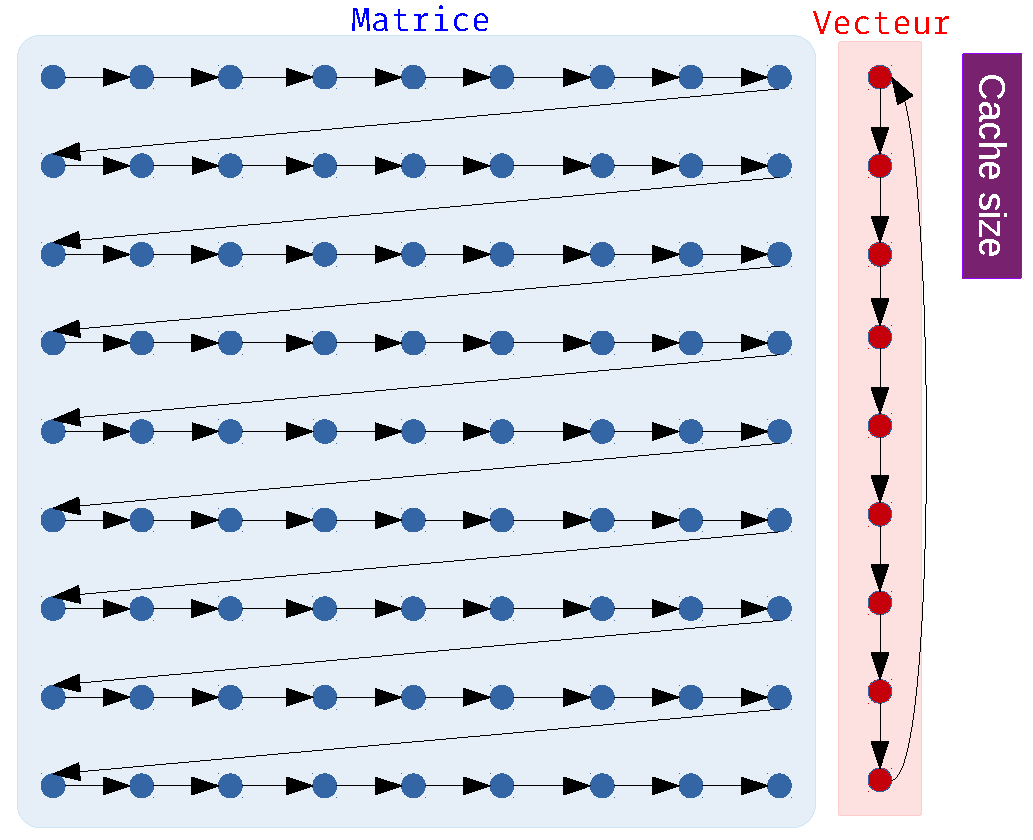
\includegraphics[width=\linewidth]{images/tiling1}
        \end{minipage}
        \begin{minipage}{0.05\linewidth}
            \center
            $\rightarrow$
        \end{minipage} 
        \begin{minipage}{0.45\linewidth}
            \center
            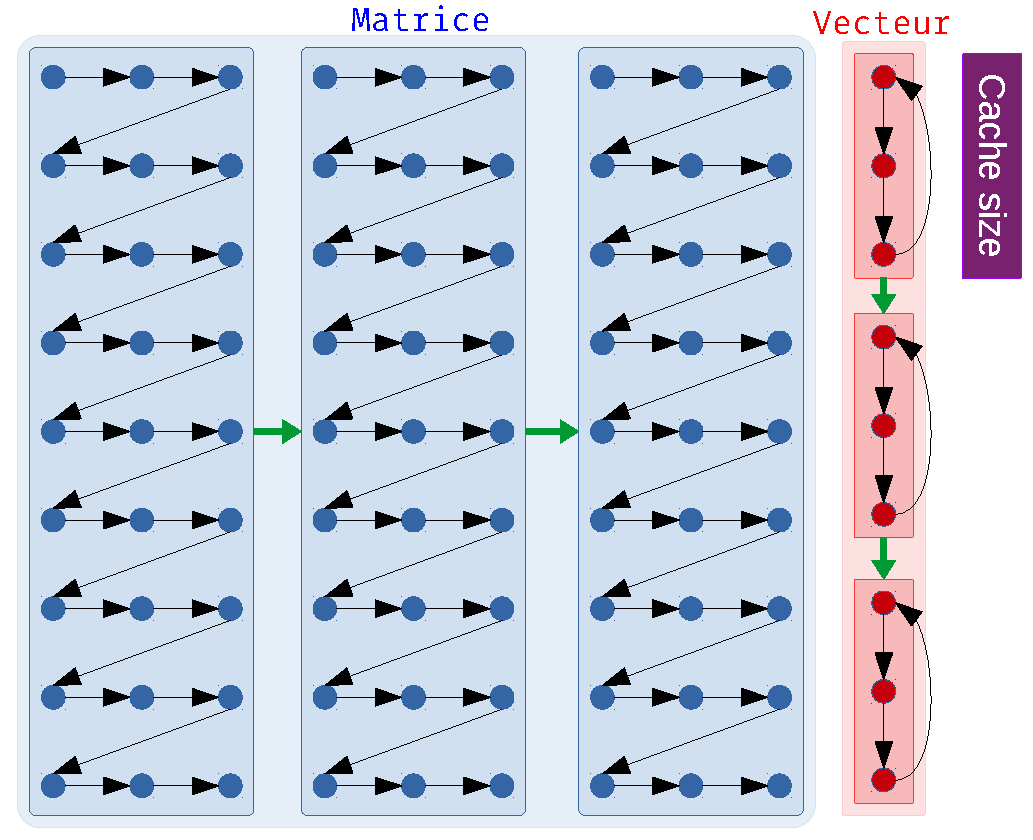
\includegraphics[width=\linewidth]{images/tiling2} 
        \end{minipage}

    \end{frame}
    \begin{frame}{Tiling Hyperplane}
        %\pause
        Un Tiling Hyperplane $\Rightarrow$ guide des transformations de boucle débloquant le tiling.
        \bigskip

        Pluto calcule les Tiling Hyperplane optimaux selon son algorithme.
        \vspace{-1.2em}
        \begin{itemize}\itemsep0em
            \item Ce Tiling Hyperplane caractérise un statement (selon Pluto)
            \item Le profil = Tiling Hyperplane calculé par Pluto.
        \end{itemize}


    Affinité : $1.0$ si égalité des Tiling Hyperplanes, $0.0$ sinon.
    \end{frame}


    
\section{Stratégie d'agrégation de statements}
    \begin{frame}{SSAA : Successive Statement Aggregation Algorithm}
        Fonctionnement du SSAA :
        \vspace{-1em}
        \begin{itemize}
            \item Ordre d'agrégation : du 1er au dernier statement
            \item Condition d'agrégation de 2 statements :
            \pause
                \begin{itemize}
                    \item Être successif.
                    \item Avoir la même \textit{Domain Matrix}
                    \item Avoir la même profondeur de boucle
                    \item Avoir une note d'affinité supérieure au minimum.
                \end{itemize}
        \end{itemize}
        \pause
        
        Note d'affinité $ = $ Moyenne pondérée des notes d'affinité des profils.

    \end{frame}
    %\begin{frame}{Futures stratégies d'agrégation}
    %\end{frame}


%\section{Agrégation de profils et statements}
    \begin{frame}{Agrégation de profils et statements}

        Agrégation des profils :
        \vspace{-1.1em}
        \begin{itemize}\itemsep0em
        \item Profil de réutilisation : fusion des groupes
        \item Profils de Parallélisme \& Vectorisation : intersection des listes de boucles
        \item Profil de Tiling Hyperplane : re-calcul par Pluto.
        \end{itemize}

        \bigskip
        
        Agrégation des statements en OpenScop :
        \vspace{-1.1em}
        \begin{itemize}\itemsep0em
            \item \textbf{Agrège 2 statements en un seul}
            \item Concatène le code textuel
            \item \textbf{Retire les \textit{Access Relations} redondantes}.
        \end{itemize}
    \end{frame}

\section{Experimentation \& Benchmarks}
    \begin{frame}{\currentname}
        SuBStrAte : the Similar Behaving Statement Aggregator.
        \bigskip
       
        Programmes benchmarkés :\\
        PolyBench 4.1, conventional\_beamforming.c.
        \pause

        \bigskip

        Benchmarks effectués :
        \vspace{-1.5em}
        \begin{itemize}\itemsep0em
            \item Nombre de statements agrégés par Substrate
            \item Speedup de Pluto
            \item Speedup des programmes.
        \end{itemize}
        \vspace{-1em}
        Le tout par note d'affinité minimale, en mono-critère avec SSAA.
        

    \end{frame}
    \begin{frame}{Résultats des benchmarks}
        \only<1>{
        Nombre de statements agrégés par Substrate (SSAA, mono-critère) :
        %\vspace{-1.5em}
        \begin{itemize}\itemsep0em
            \item 8/31 programmes affectés
            \item Agrégation même avec note d'affinité élevée (\textasciitilde0.6)
            \item Résultats à comparer avec les benchmarks de speedup.
        \end{itemize}
        \vspace{-1.5em}
        \begin{center}
        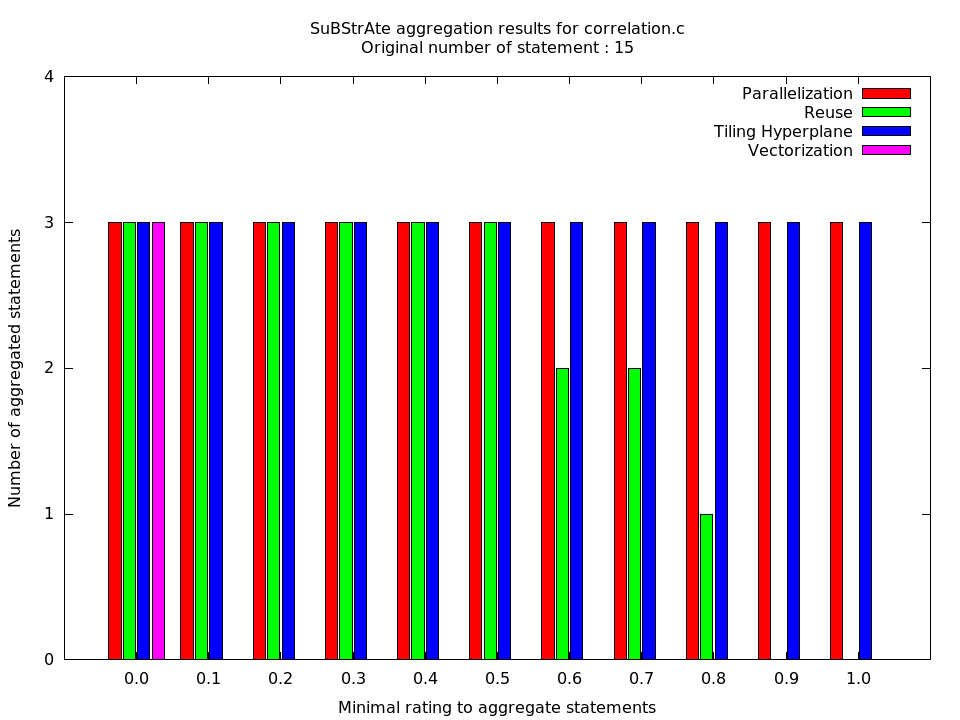
\includegraphics[width=0.72\linewidth]{images/results/correlation}
        \end{center}
        }

        \only<2>{
        Speedup de Pluto :
        %\vspace{-1.5em}
        \begin{itemize}\itemsep0em
            \item Agrégation $\Rightarrow$ Speedup de Pluto (pour tout programmes benchmarkés)
            \item Moyenne à environ 1.2, pics à 1.5 et 1.9 .
        \end{itemize}
            \begin{minipage}{0.499\linewidth}
                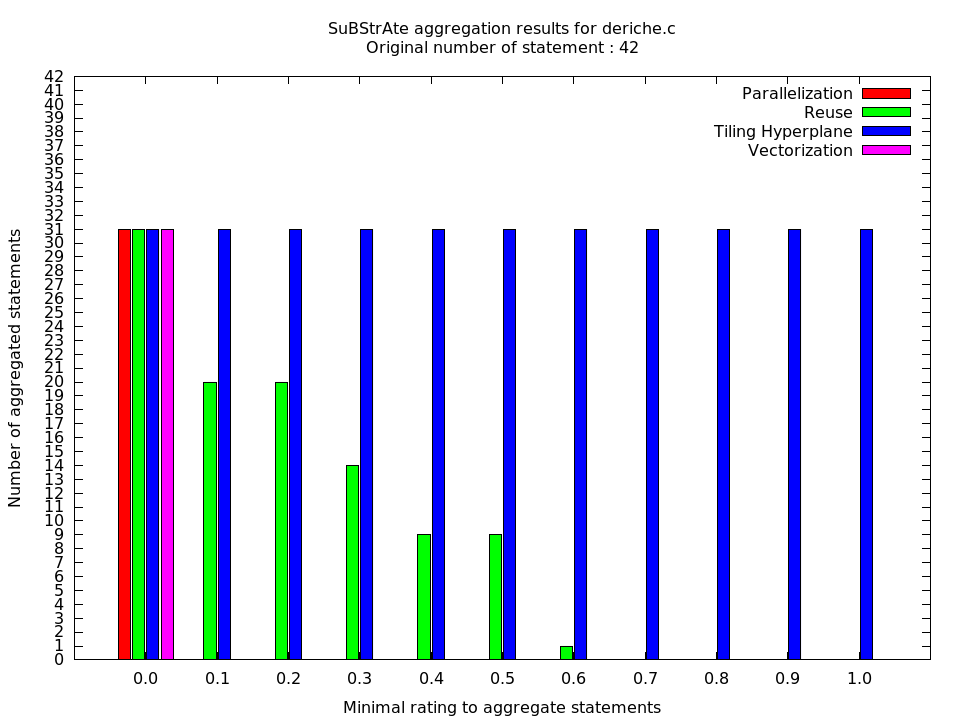
\includegraphics[width=\linewidth]{images/results/deriche1}
            \end{minipage}\hfill
            \begin{minipage}{0.499\linewidth}
                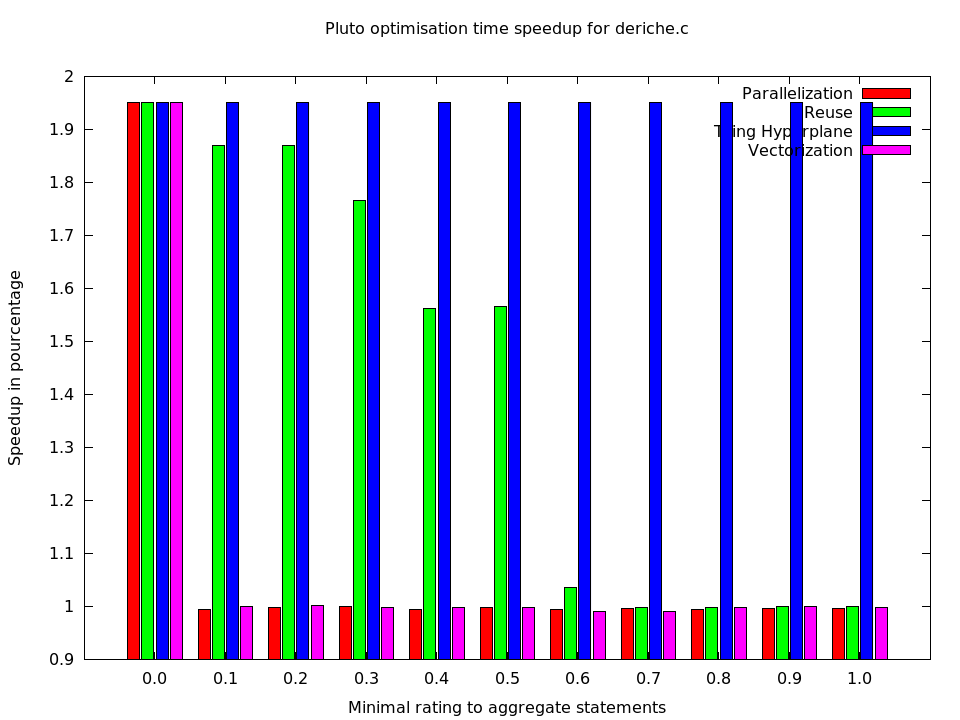
\includegraphics[width=\linewidth]{images/results/deriche2}
            \end{minipage}
        }

        \only<3>{
        Speedup des programmes :
        %\vspace{-1.5em}
        \begin{itemize}\itemsep0em
        \item 3/8 programmes affectés montrent un speedup
        \item conventional\_beamforming.c : speedup de 1.5 en moyenne
        \item correlation.c : speedup de 1.7 en moyenne
        \item covariance.c : speedup de 1.65 en moyenne.
        \end{itemize}
            \begin{minipage}{0.499\linewidth}
                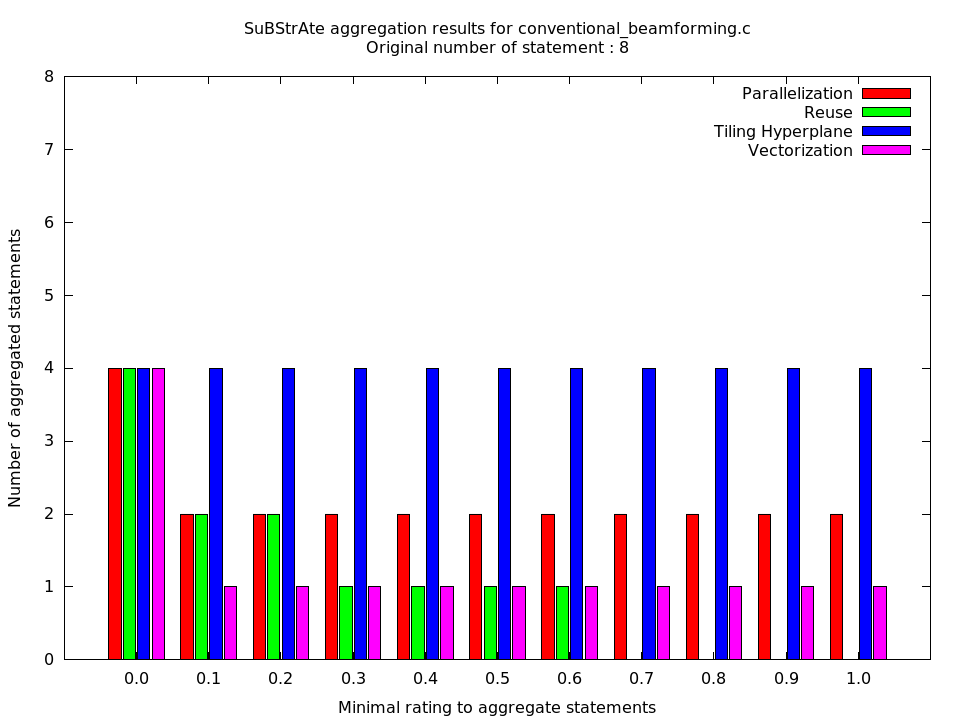
\includegraphics[width=\linewidth]{images/results/conventional_beamforming1}
            \end{minipage}\hfill
            \begin{minipage}{0.499\linewidth}
                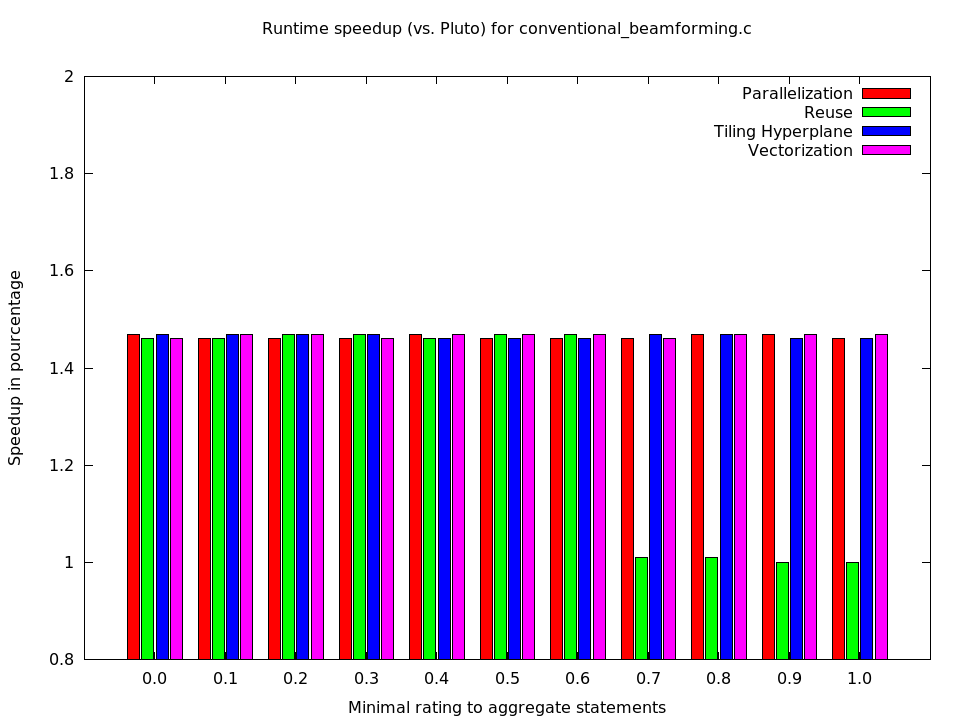
\includegraphics[width=\linewidth]{images/results/conventional_beamforming2}
            \end{minipage}
        }
    \end{frame}

%Optionnelle
%\section{Future Works}
    %\begin{frame}{\currentname%→ Additional Profil Type
%→ Additional Aggregation Strategies
%→ Statement different cuting
    %\end{frame}

\section{Conclusion}
    \begin{frame}{\currentname}
        Résultats très encourageants :
        \vspace{-1em}
        \begin{itemize}
            \item Agrégation utile ou peu nuisibe (code court)
            \item Agrégation = speedup optimisateur
            \item Agrégation → débloque meilleurs optimisations.
        \end{itemize}

        Fonctionne bien avec certaines classes de code\\(ex. : détection de radar).

        \pause

        \textbf{Il reste encore 1 mois de stage !}
        \begin{itemize}
            \item Écriture de benchmarks supplémentaires
            \item Implémentation nouvelles stratégies d'agrégation
            \item Implémentation du profile de \textbf{pression de registre}.
        \end{itemize}
    \end{frame}

    \begin{frame}{\currentname}
        Retour sur le stage :
        \pause
        \begin{itemize}
            \item \alert<+>{Début lent}
            \item \alert<+>{Gestion du temps de travail et questions}
            \item \alert<+>{Apprentissage de techniques d'optimisation}
            \item \alert<+>{Modèle polyédrique "élégant"}
            \item \alert<+>{Introduction au monde de la recherche }
            \item \alert<+>{Parler en anglais.}
        \end{itemize}
        
        \pause

        En résumé : des hauts et bas, mais ce fut une \textbf{experience enrichissante et formatrice}.
    \end{frame}

\plain{Merci de votre attention.\\Avez vous des questions?}
\end{document}
